\section{Statistical Uncertainties}\label{sec:results.staterrors}

In this section, the calculations leading up to the statistical uncertainty of the cross-section measurement will be discussed. Statistical fluctuations of the measurement will depend solely on the variables in eq.~\ref{eq:xsection2} that are not constant and can vary depending on bin width or calculation methods. For this analysis, discrete binning was employed allowing to utilize Poisson distribution error estimation. A Poisson distribution $P(\lambda,k)$ is defined as,
\begin{equation}
P(\lambda,k) = \frac{\lambda^k e^{-\lambda}}{k!}
\end{equation}
with $k$ being the observed occurrences, $\lambda$ being the rate of occurrences and also the variance, is a discrete probability distribution that expresses the probability of a given number of events occurring in a fixed interval of time and/or space if these events occur with a known average rate and independently of the time since the last event~\cite{Poisson}. With $\lambda$ as the variance of the measurement the standard deviation ($\sigma$), or error of the measurement is described by $\sigma = \sqrt{\lambda}$. 
For data samples of uncorrelated variables, the error propagation can be described as
\begin{equation}
\left(\frac{\sigma_f}{f}\right)^2 = \sum_{i=1}^{M}\left(\frac{\sigma_i}{f_i}\right)^2
\end{equation}

Let's denote the differential cross-section as 
\begin{align}
\frac{d\sigma}{d\cos\theta^{\pi^0}_{C.M.} d\phi} = \varXi \nonumber
\end{align}
and the error of $\varXi$ to be
\begin{align}
\sigma_\varXi = \varXi \left(\left(\frac{\sigma_{\Upsilon}}{\Upsilon}\right)^2 +\left(\frac{\sigma_{ \eta(E_\gamma,\cos\theta^{\pi^0}_{C.M.})}}{\eta(E_\gamma,\cos\theta^{\pi^0}_{C.M.})}\right)^2 + \left(\frac{\sigma_{F(E_\gamma)}}{F(E_\gamma)}\right)^2\right)^{\frac{1}{2}}\label{eq:xsection.error}
\end{align}
where the statistical error of the flux $F(E_\gamma)$ and detected particles $\Upsilon$ is given by Poisson statistics,
\begin{subequations}
\begin{align}
\sigma_{F(E_\gamma)} = \sqrt{F(E_\gamma)} \label{eq:flux.err} \\
\sigma_{\Upsilon} = \sqrt{\Upsilon} \label{eq:yield.err}. 
\end{align}
\end{subequations}
From eq.~\ref{eq:acceptance}
\begin{align}\label{eq:acceptance.error}
\left(\frac{\sigma_\eta}{\eta}\right) = \left(\left(\frac{\sigma_R}{N_R}\right)^2 +\left(\frac{\sigma_G}{N_G}\right)^2\right)^{\frac{1}{2}}
\end{align}
where the statistical error of the reconstructed events, $\sigma_R$, and generated events, $\sigma_G$, is given by Poisson statistics
\begin{subequations}
\begin{align}
\sigma_{R} = \sqrt{N_R} \nonumber\\
\sigma_{G} = \sqrt{N_G} \nonumber
\end{align}
\end{subequations}
therefore 
\begin{align}\label{eq:acceptance.error.simp}
\left(\frac{\sigma_\eta}{\eta}\right) = \left(\frac{1}{N_R} +\frac{1}{N_G}\right)^{\frac{1}{2}}
\end{align}
The number of events reconstructed, $N_R$ for the simulation was chosen to be such that $N_R \sim 4\Upsilon$, while the pair-production rate combined with the acceptance made it such that $N_R \ll N_G$, simplifying eq.~\ref{eq:acceptance.error.simp} to be
\begin{align}\label{eq:acceptance.error.simpII}
\left(\frac{\sigma_\eta}{\eta}\right) = \left(\frac{1}{4\Upsilon}\right)^{\frac{1}{2}}.
\end{align}
It should also be noted that the beam energy binning chosen reflects that $\Upsilon \ll F(E_\gamma)$ and so substituting Eqs.~\ref{eq:yield.err},~\ref{eq:flux.err},~\ref{eq:acceptance.error.simpII} into Eq.~\ref{eq:xsection.error} yields
\begin{align}
\sigma_\varXi = \varXi \left(\frac{1}{\Upsilon} +\frac{1}{4\Upsilon}\right)^{\frac{1}{2}}\label{eq:xsection.error.part1}
\end{align}
The backward angle binning discussed in Sec~\ref{sec:results.xsection} eq.~\ref{backbin} was chosen to minimize the statistical error by maximizing 
\begin{align}
\left(\frac{1}{\Upsilon} +\frac{1}{4\Upsilon}\right)^{\frac{1}{2}}\label{eq:xsection.error.part}
\end{align}
The contribution of eq.~\ref{eq:xsection.error.part} is shown in Fig.~\ref{fig:results.staterr} for values of $\Upsilon < 100$ which is typical at high beam energies, large backward $cos\theta^{\pi^0}_{C.M.}$.

\begin{figure}[h!]\begin{center}
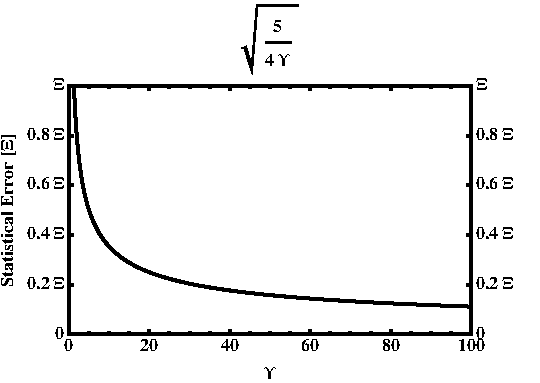
\includegraphics[width=\figwidth,height=\qfigheight]{\figures/analysis/statistical_errorII.pdf}
\caption[The uncertainty plotted vs. the total number of detected events and reconstructed events from \abbr{MC}, for small values of $\Upsilon$]{\label{fig:results.staterr}The uncertainty plotted vs. the total number of detected events and reconstructed events from \abbr{MC}, for small values of $\Upsilon$. The binning in the backward direction was chosen to maximize $\Upsilon$ to reduce the overall statistical error }
\end{center}\end{figure}

\FloatBarrier